\section{EXPERIMENTAL RESULTS}
In this section, we show the experimental results to verify the proposed power budgeting method and analyze its energy efficiency and performance. All data are collected on a PC with Intel I5 2400 CPU and 4 GB memory. Multi-core systems with core number ranging from $9$ to $100$ are used in the experiment, and each core with different dark silicon ratio are tested. The thermal models of these multi-core systems are extracted from HotSpot with default package and chip parameters. The ambient temperature are set to be \SI{20}{\degreeCelsius} for all test cases, and the temperature constraint is \SI{80}{\degreeCelsius}.


\begin{figure}
  \centering
  \subfigure[The first step with position and power budget of the first active core determined.]{
    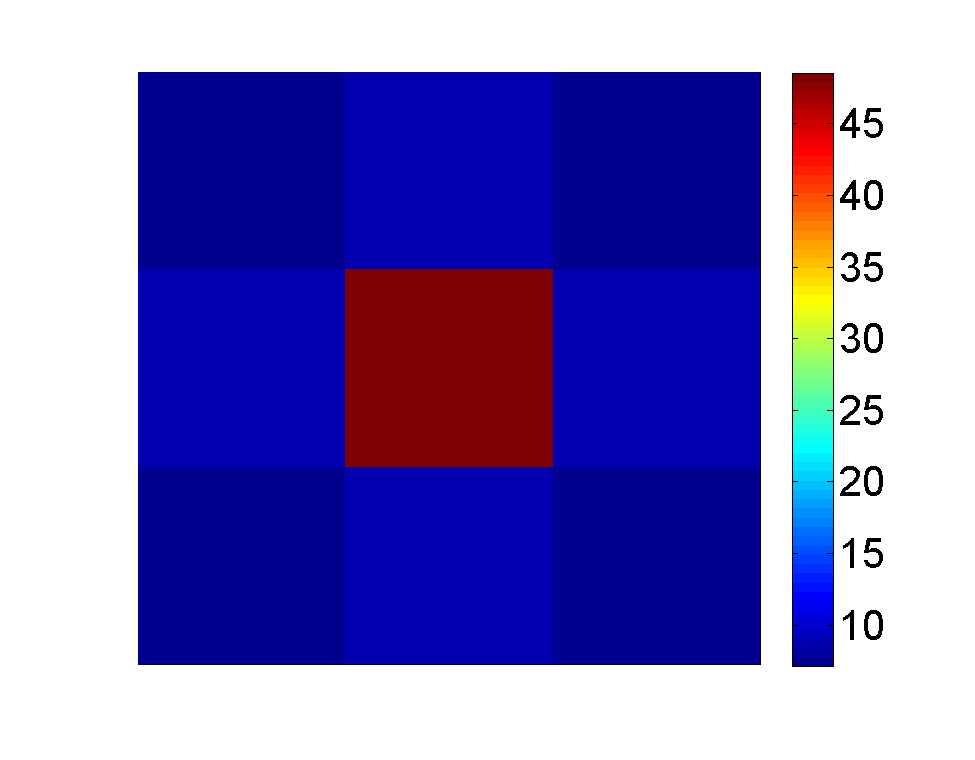
\includegraphics[width=0.46\columnwidth]{fig/order_of_cores_1.eps}\label{fig:order_of_cores_1}
  }
  \hfill
  \subfigure[The second step with positions and power budgets of 2 active cores determined.]{
    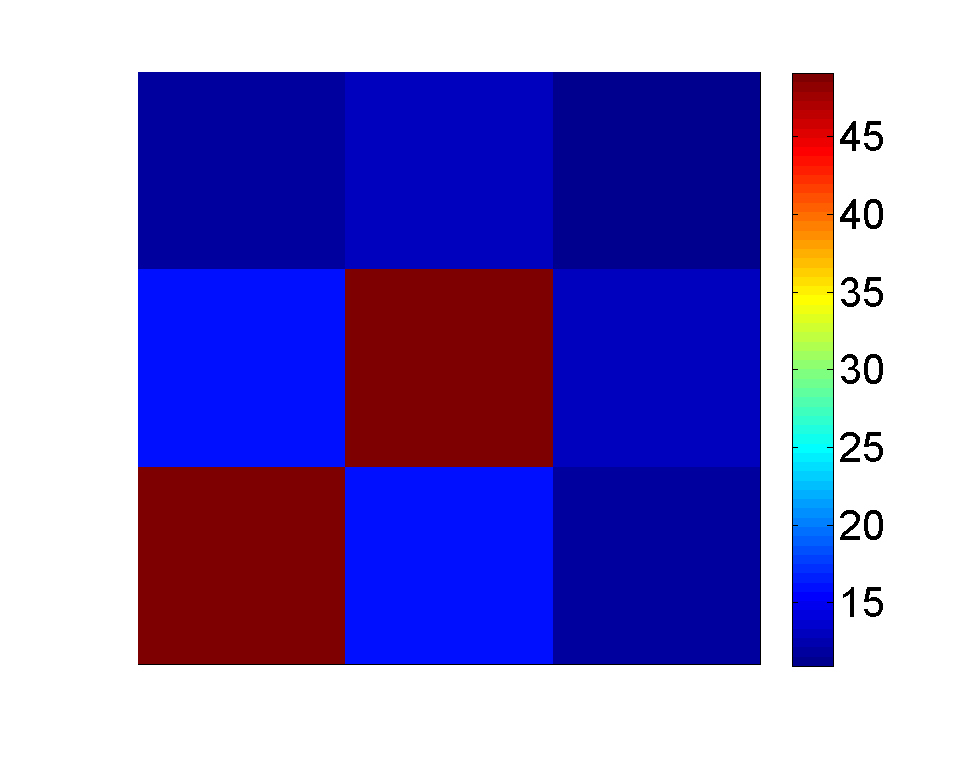
\includegraphics[width=0.46\columnwidth]{fig/order_of_cores_2.eps}\label{fig:order_of_cores_2}
  }
  \subfigure[The third step with positions and power budgets of 3 active cores determined.]{
    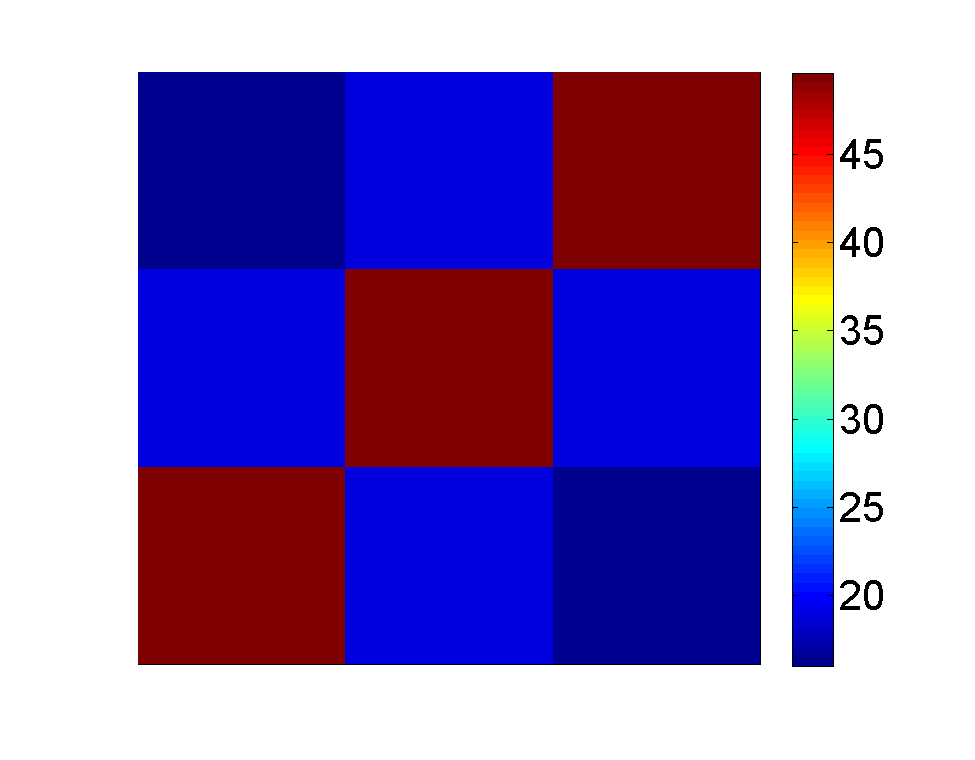
\includegraphics[width=0.46\columnwidth]{fig/order_of_cores_3.eps}\label{fig:order_of_cores_3}
  }
  \hfill
  \subfigure[The fourth step with positions and power budgets of 4 active cores determined.]{
    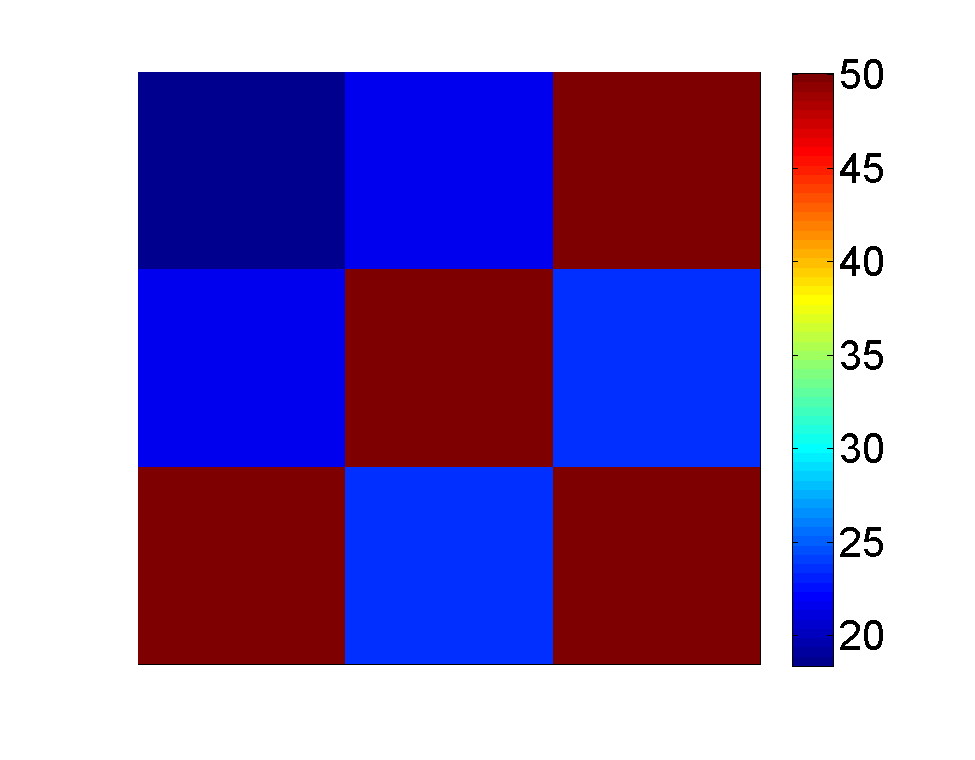
\includegraphics[width=0.46\columnwidth]{fig/order_of_cores_4.eps}\label{fig:order_of_cores_4}
    }
  \caption{Temperature distributions of the 9-core system with the power budget given by our method's first four greedy steps.}
  \label{fig:order_of_cores}
\end{figure}

\subsection{Effectiveness and energy efficiency test for steady state cases}
In order to test the effectiveness and performance of the new method, we first test it
using a system with small core number ($9$ cores) and show its steady state
behavior step in step. Please note that we show steps of the $9$-core system
because it is easier for the readers to verify the correctness of GDP using
a system with small core number.

Now we demonstrate how our method decides which cores to be active in a
greedy manner for $4$ active cores. For step one, our method looks for the first
active core position. This step is pretty easy even for human, as we
can readily pick the center core, because its position has the best
heat dissipation capability. GDP, unlike human who uses instinct and
experience, picks the core with the highest performance under $\hat{T}_{opt}$, which is exactly the center core. 
Then, our method computes the power
budget for such one active core case. We plot the steady state temperature
distribution caused by the computed power budget in
Fig.~\ref{fig:order_of_cores_1}. As expected, the only active core at
the center has a temperature of \SI{48}{\degreeCelsius}, which is just
the computed optimal temperature for it. Next, our method searches for the
second active core position with the first active core position
fixed. Although all four cores at the corners can be chosen due to
symmetry, the upper left one is picked simply because computer prefers
the first. The updated power budget also leads to
$\hat{T}_{opt}$ for the two active cores shown in Fig.~\ref{fig:order_of_cores_2}, as expected. For the
third and fourth active cores, GDP locates their positions to be 
lower right corner and upper right corner, with power budget
resulted temperature distributions shown in
Fig.~\ref{fig:order_of_cores_3} and Fig.~\ref{fig:order_of_cores_4}. Note that the difference between optimal temperature for different cores is within \SI{2}{\degreeCelsius} in our case.



\begin{table}
%  \color{red}
  \caption{Energy efficiency (in MIPS/Watt) results comparison of steady state power budgeting. "New" stands for our new power budgeting method, "Monte Carlo" denotes the optimal result with maximum PPW from $10000$ Monte-Carlo simulation with varables being active core distribution and DVFS stage of each active core.}
  \label{tab:PPW_steady}
  \centering
  \begin{tabular}{c|c||c|c}
    \hline
    Core & Active     & \multirow {2}{*}{New} &
                                                    \multirow {2}{*}{Monte-Carlo }\\

\#       &   \#       & &   \\
%\#      &   \#         & (W)        &      &   (W)   &    &  (W)    &    &(W)   &  (W)\\
     \hline
\hline
  \multirow{3}{*}{9} &      2     &       2.8       & 3.0   \\ 
             &      4             &      2.6     &  2.6  \\
             &      7             &       2.4     &  2.3  \\
     \hline
\multirow{3}{*}{16}   &      3    &      2.6     &   2.9 \\   
             &      8             &      2.6    &   2.6  \\
             &      13            &      2.3     &   2.1\\
     \hline
 \multirow{3}{*}{25}  &      5    &     2.8    &   3.0     \\ 
                &     12          &     2.8   &   2.7    \\
                &     20          &     2.7    &   2.5    \\
     \hline
  \multirow{3}{*}{36}  &     8            &      2.8    &  2.9     \\
              &     18            &     2.7          &  2.6   \\
              &     28          &        2.6         &  2.4  \\
     \hline
 \multirow{3}{*}{64}   &     12           &     2.7  &   2.8    \\
              &     32      &      2.8           &   2.7    \\
              &     52        &      2.4          &   2.3     \\
              
 \hline 
 \multirow{3}{*}{100} & 16 & 2.8  &   2.7   \\
                      & 52 & 2.7  &   2.5  \\
                      & 76 & 2.4  &  2.3   \\
\hline
  
\end{tabular}
\end{table}



Due to the high computational complexity of the problem, the optimal active core distribution and the corresponding DVFS stage of each active core for maximum energy efficiency through brute force search is impossible to obtain for multi-core system with large core number. Therefore, in the experiment, we implement the Monte Carlo method, and compare the energy efficiency of our power budget with the optimal result from Monte Carlo method. 
% we find that the energy efficiency of our computed power budget is close to the optimal one.
\begin{figure}
\centering
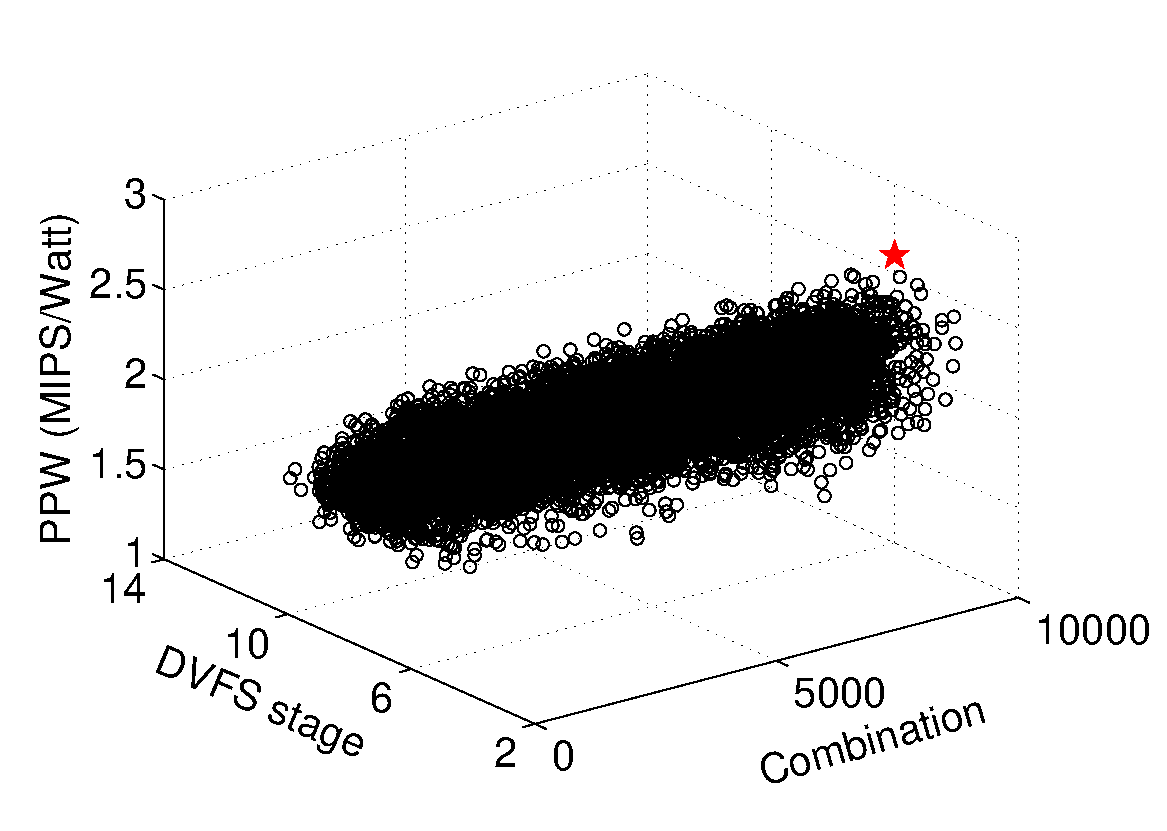
\includegraphics[width=1\linewidth]{fig/best_steady.eps}
\caption{Monte-Carlo of a $16$-core system with $8$ active cores, the variables are the active core distribution and the DVFS stage of each core, the random combination number is 10000, the red pentagram stand for the energy efficiency of our computed power budget}
\end{figure}





In addition to the case shown above, we also tested many other systems with different numbe of cores and active cores. The energy efficiency of these cases are shown in Table~\ref{tab:PPW_steady}. For all cases, the energy efficiency of our given power budget is close to the optimal result.





\begin{table}
%  \color{red}
  \caption{Energy efficiency (in MIPS/Watt) and system performance (in MIPS) results comparison of steady state power budgeting. "New" stands for our new power budgeting method, "Random" denotes the averaged result from $10$ random active core distribution with $T_{opt}$ reached for each active core.}
  \label{tab:PPW_perf_steady}
  \centering
  \begin{tabular}{c|c||c|c||c|c}
    \hline
    Core & Active     & \multicolumn{2}{c||}{New} &
                                                     \multicolumn{2}{c} {Random}\\
\cline{3-6}  
\#       &   \#        & PPW & Perf   & PPW  & Perf \\
%\#      &   \#         & (W)        &      &   (W)   &    &  (W)    &    &(W)   &  (W)\\
     \hline
\hline
  \multirow{3}{*}{9} &      2     &       2.8    & 137.1     & 2.8 & 122.0\\ 
             &      4             &      2.6     & 222.4     & 2.6 & 211.5\\
             &      7             &       2.4    & 290.2      & 2.4 & 272.3\\
     \hline
\multirow{3}{*}{16}   &      3    &      2.6     & 130.0    &  2.6 & 113.5\\   
             &      8             &      2.6    & 243.3    & 2.5 & 225.3 \\
             &      13            &      2.3     &  270.6   &  2.3 & 252.9\\
     \hline
 \multirow{3}{*}{25}  &      5    &     2.8   &  131.7    & 2.8 &115.8       \\ 
                &     12          &     2.8   &   232.3  & 2.8  & 220.3    \\
                &     20          &     2.7   &   271.2    & 2.7 & 249.5 \\
     \hline
  \multirow{3}{*}{36}  &     8            &      2.8   & 142.0    &  2.8  &124.0    \\
              &     18            &     2.7         & 228.9   &  2.7  & 215.6 \\
              &     28          &        2.6      &   263.2     &  2.6 & 242.2 \\
     \hline
 \multirow{3}{*}{64}   &     12           &     2.7  & 132.2   &     2.7   & 117.7  \\
              &     32      &      2.8      &     230.7     &    2.8   & 216.2  \\
              &     52        &      2.4       & 245.7       &  2.4   & 232.6   \\
              
 \hline 
 \multirow{3}{*}{100} & 16 & 2.8 &  122.6    &   2.8   &   109.1  \\
                      & 52 & 2.7 &  242.1     &   2.7   &   226.5  \\
                      & 76 & 2.4 &  285.7     &   2.4   &   267.8  \\
\hline
  
\end{tabular}
\end{table}


Next, we test the power budget quality provided by our method. The results are collected in Table~\ref{tab:PPW_perf_steady}. For comparison, we randomly generate $10$ active core distribution for each case, and compute the averaged energy efficiency and averaged performance with the $T_{opt}$ reached for each active core. As the Table~\ref{tab:PPW_perf_steady} shows, our method provides the optimal performance while the energy efficiency is maximized.





% \begin{figure*}[htbp]
% \centering
% \begin{minipage}[c]{0.5\textwidth}
% \centering
%   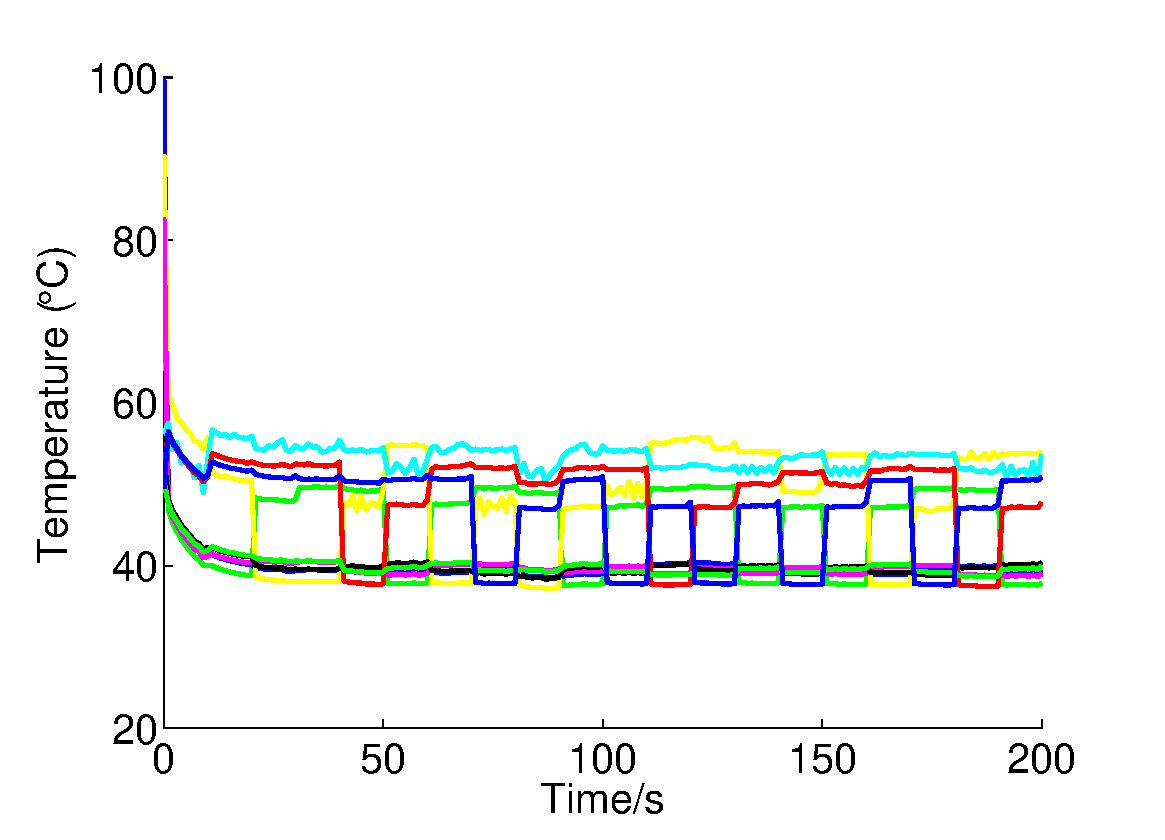
\includegraphics[width=6.5cm]{fig/tem_own.eps}
% \end{minipage}%
% \begin{minipage}[c]{0.5\textwidth}
% \centering
%   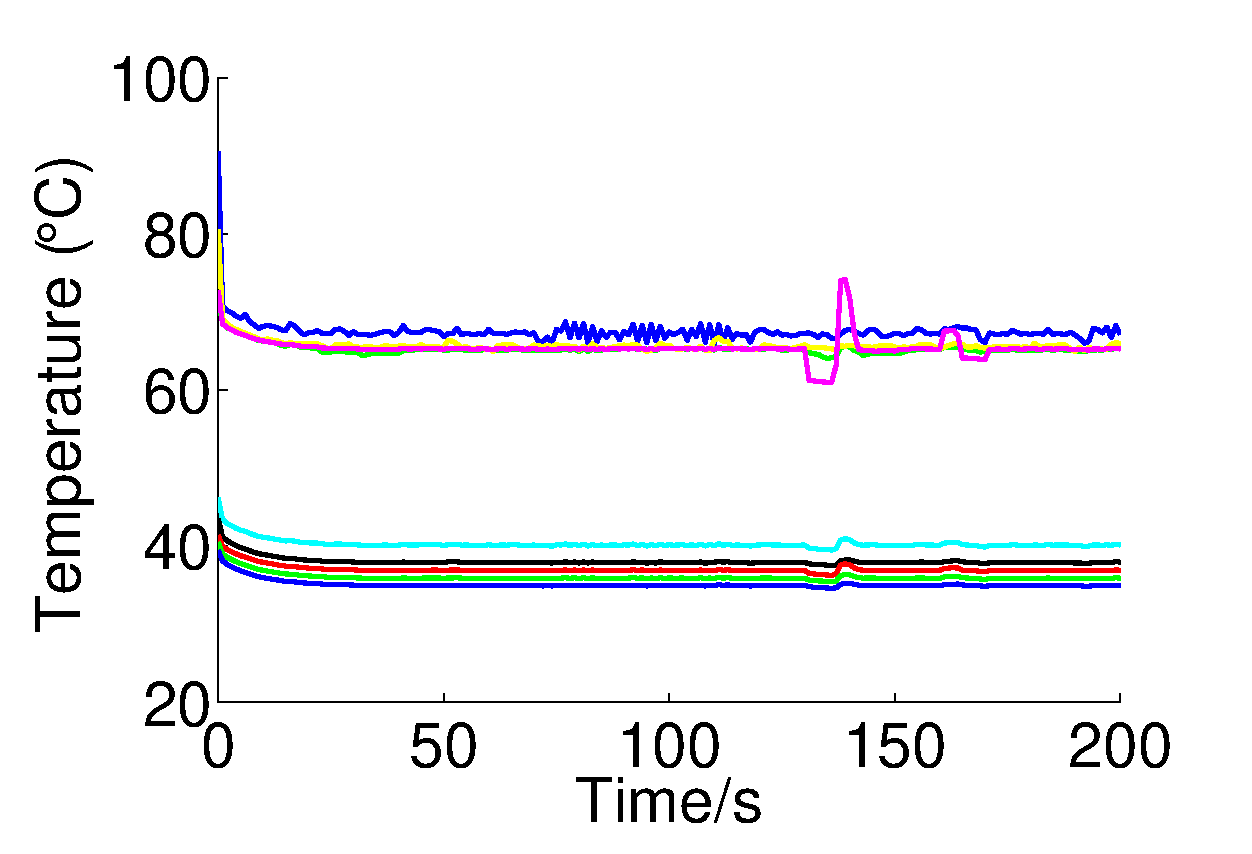
\includegraphics[width=6.5cm]{fig/tem_mag.eps}
% \end{minipage}
% \begin{minipage}[c]{0.5\textwidth}
% \centering
%   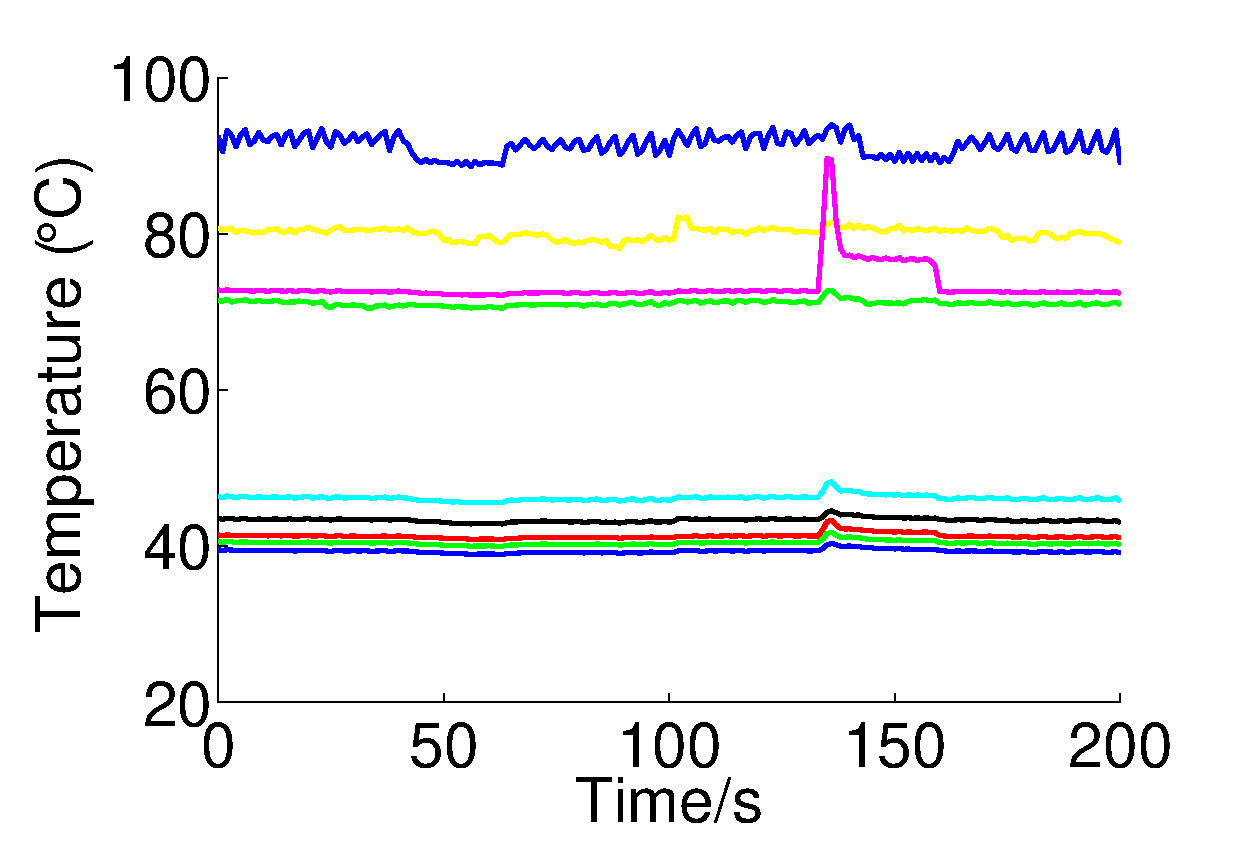
\includegraphics[width=6.5cm]{fig/tem_free.eps}
% \end{minipage}%
% \begin{minipage}[c]{0.5\textwidth}
% \centering
%   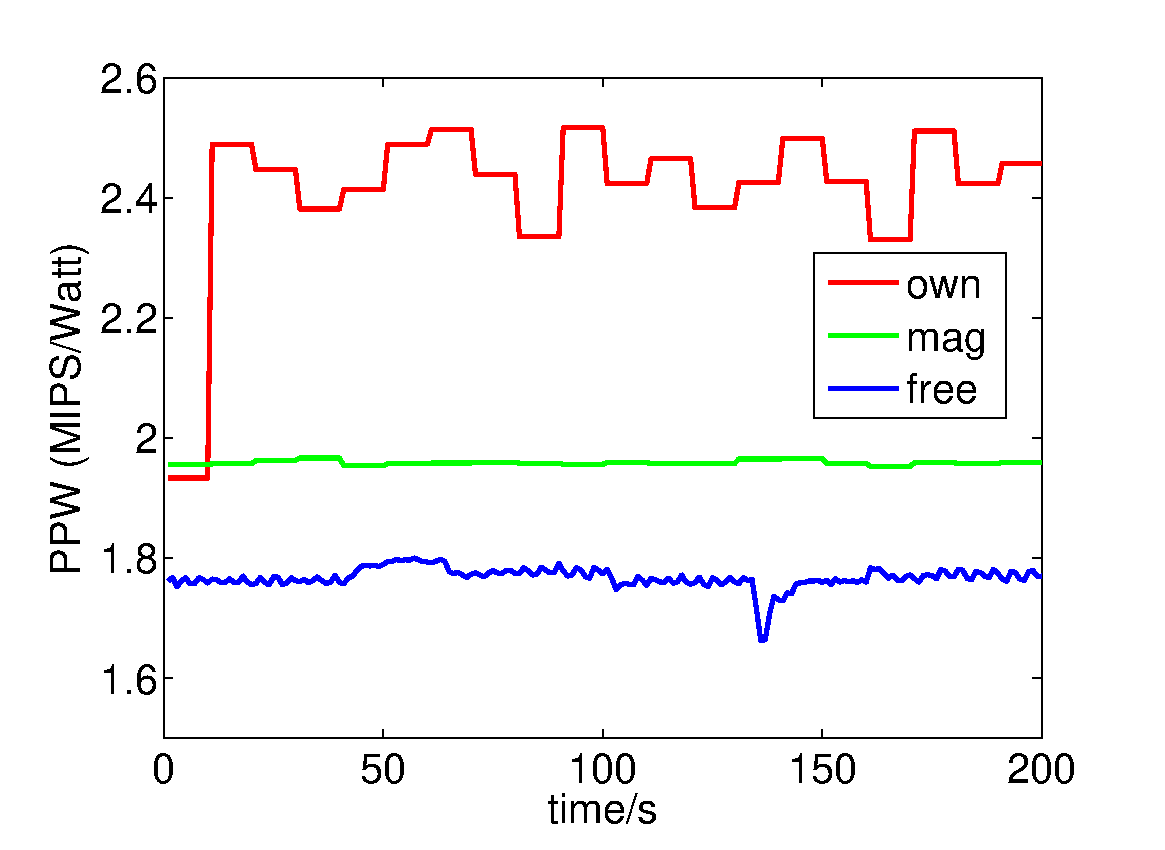
\includegraphics[width=6.5cm]{fig/PPW.eps}
% \end{minipage}
% \caption{fft}\label{fig:fft}
% \end{figure*}



\begin{figure}
  \centering
  \subfigure[Transient temperatures of the system with power budget provided by new method. The cores are activated according to the sub-optimal distribution given by our method.]{
    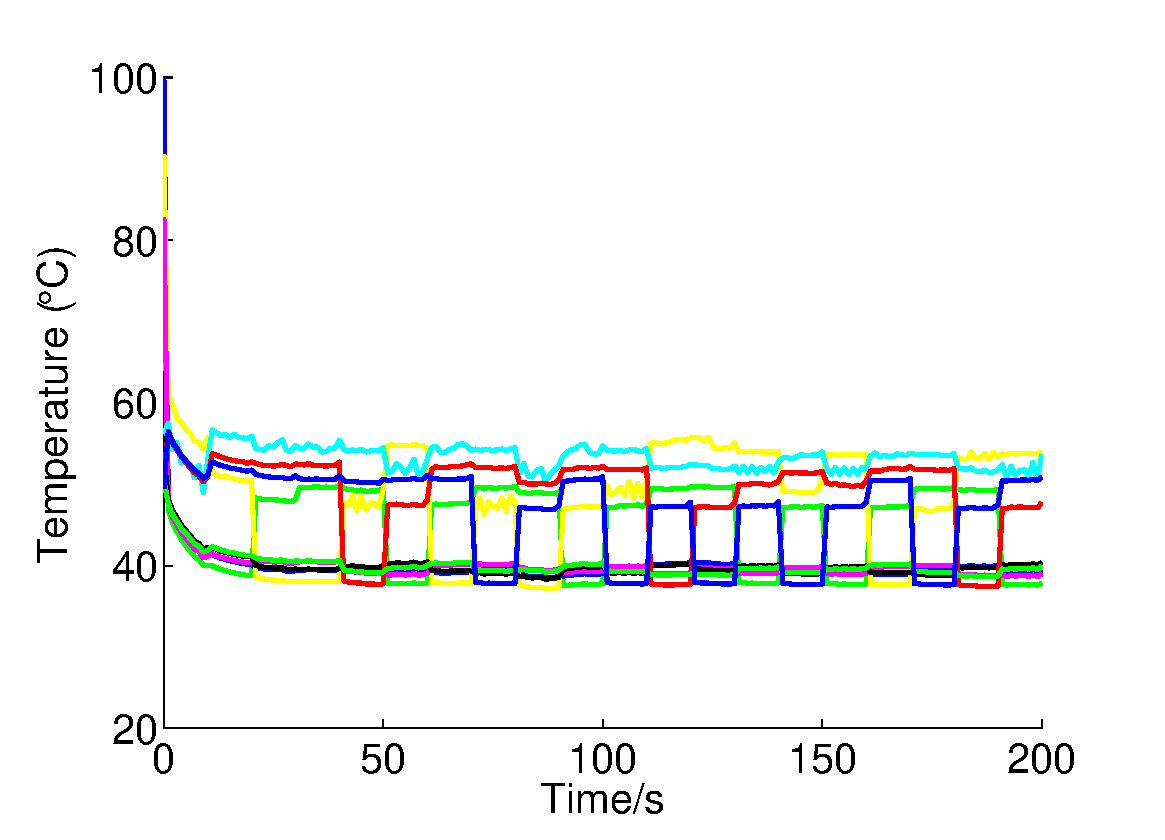
\includegraphics[width=0.45\columnwidth]{fig/tem_own.eps}\label{fig:tem_own}
  }
  \hfill
  \subfigure[Transient temperatures of the system with power budget provided by existing method. The cores with higher benefit are activated.]{
    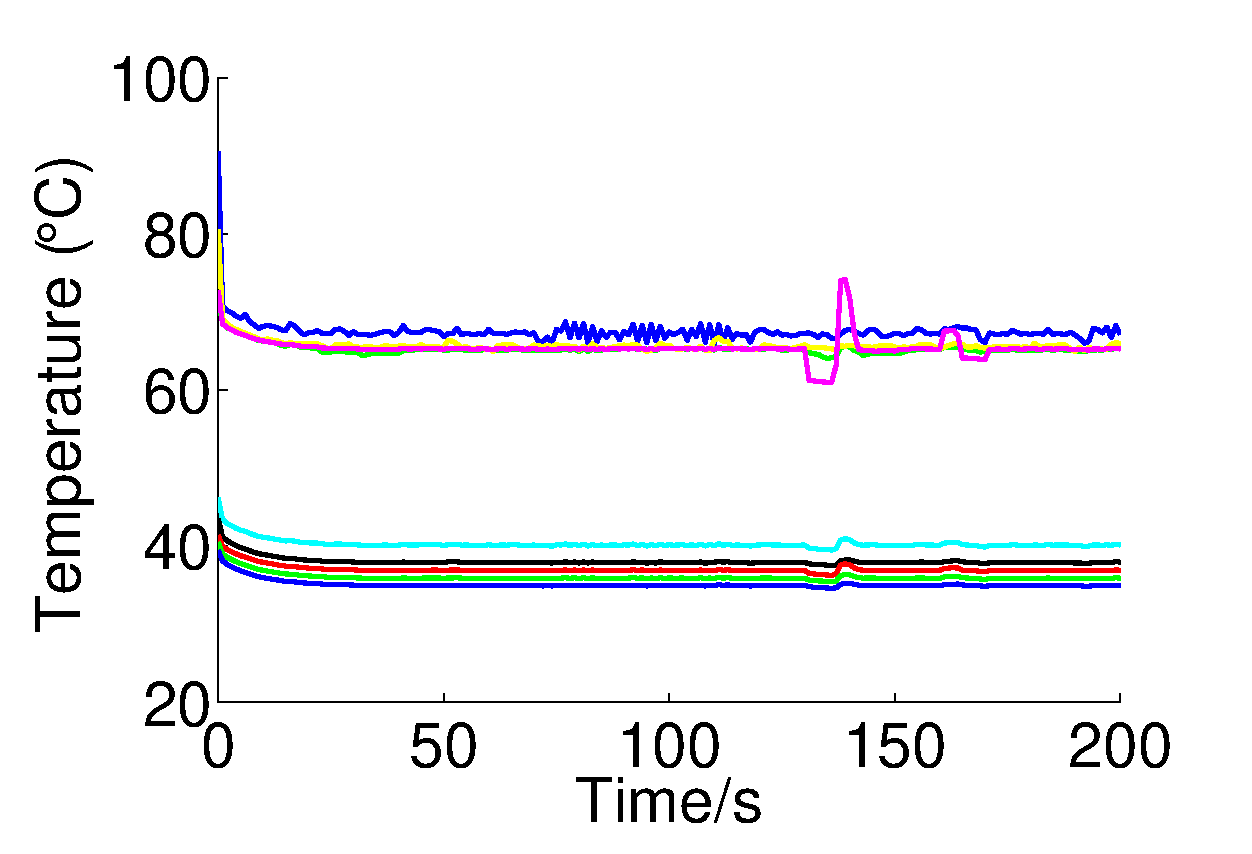
\includegraphics[width=0.45\columnwidth]{fig/tem_mag.eps}\label{fig:tem_mag}
  }
  \subfigure[Transient temperatures of the system in free run. The cores are activated randomly.]{
    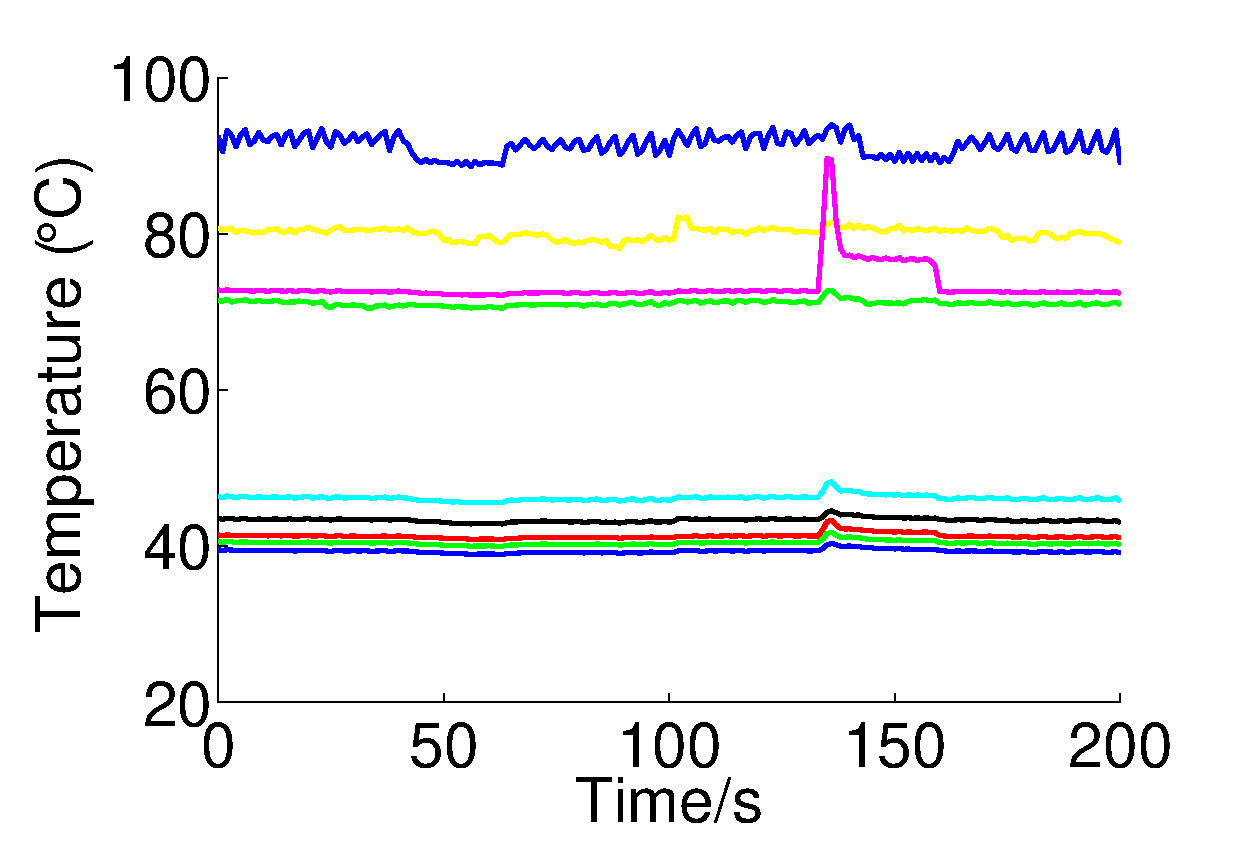
\includegraphics[width=0.45\columnwidth]{fig/tem_free.eps}\label{fig:tem_free}
  }
  \hfill
  \subfigure[The PPW curves of all $3$ cases.]{
    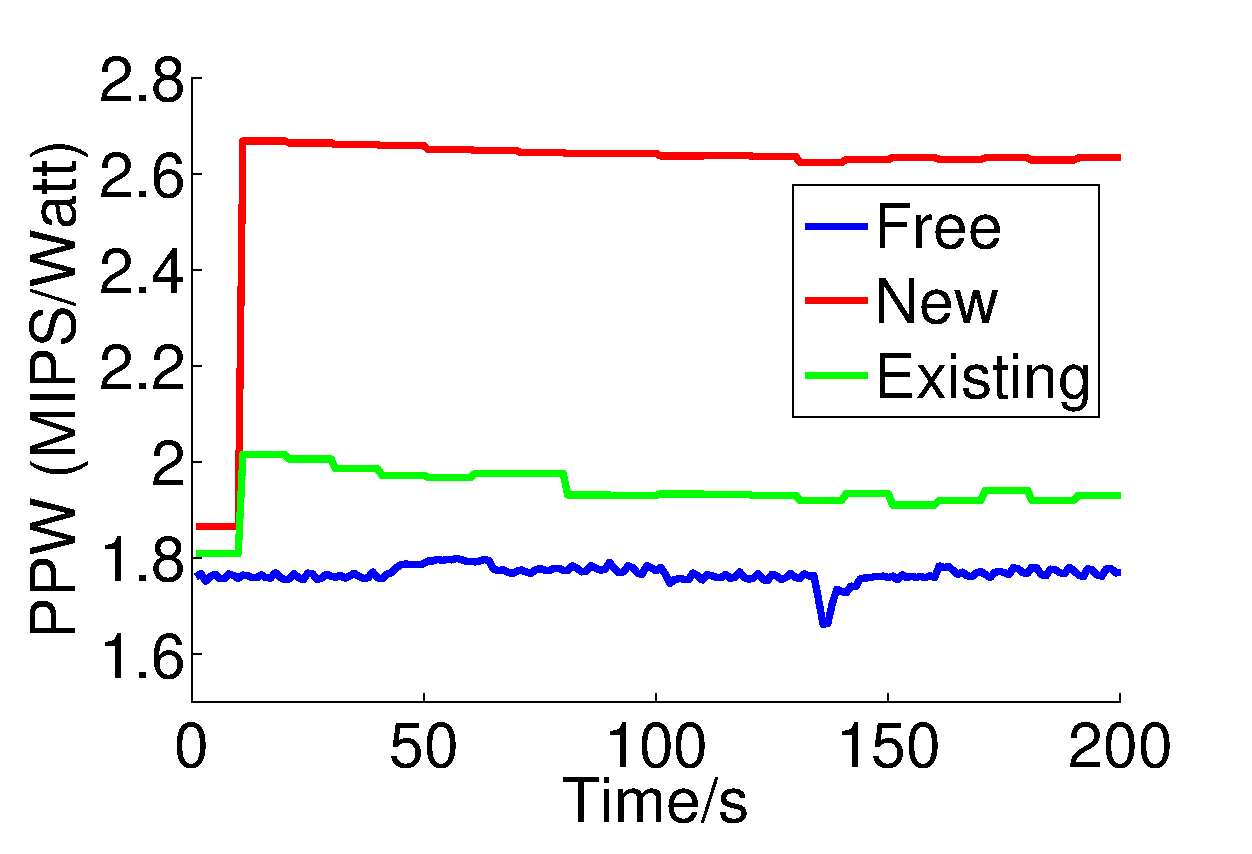
\includegraphics[width=0.45\columnwidth]{fig/PPW_new.eps}\label{fig:PPW_new}
    }
  \caption{Transient temperatures of the $9$-core system with simple task scheduling and DVFS following power budgets provided by new method, existing method and in free run. Each line represents temperature of one core of the system.}
  \label{fig:transient_ppw_temperature}
\end{figure}


\subsection{Energy-efficient power budgeting with optimal performance considering transient effects}
Our method is a dynamic based method, which means that it can provide power budget adapting to transient running state of the multi-core dark silicon system.

Our method focus on dynamically computing an energy-efficient power budget for multi-core dark silicon system. By integrating the power budget and active core distribution suggestion provided by our method, many different thermal management methods can be designed and optimized, which is not the main focus of our work. In order to verify the effectiveness of our method for transient cases, the same simple task scheduling and DVFS strategy is applied for all methods: a power matching determines task scheduling and DVFS is performed when the task on a core consumes more power than the provided power budget.

In the experiment, our method (called "new" for short) is set to compute power budget dynamically for each future second ($h=1$). State-of-art energy-efficient dynamic thermal management~\cite{Hanumaiah:TCOMP'14} (called "existing" for short)is used for comparison. The active cooling in~\cite{Hanumaiah:TCOMP'14} is neglected, and the each core power gating is introduced by choosing the cores with higher \emph{benefit} for ease of comparison without affecting the method. A case without any thermal management (called "free" for short) is also conducted for comparison. One application from SPEC benchmark is running on each active core, and the applications are randomly assigned to the active cores at the start. There are $15$ V/F levels (from $0.32$V@$200$MHz to $0.8$V@$2$GHz) for DVFS in our experiment, with DVFS action overhead set to be \SI{10}{\us} by following the settings in~\cite{Lu:MICRO'05}. The task migration overhead is set as \SI{10}{\ms} according to~\cite{Cuesta:ISVLSI'10}.

We first verify the effectiveness of new method and existing method. For the new method, as shown in Fig.~\ref{fig:tem_own}, the temperature of all active cores are constrained around \SI{48}{\degreeCelsius}, which is the $\hat{T}_{opt}$ for $9$-core system with $4$ active cores as shown in Fig.~\ref{fig:order_of_cores_4}, with the simple task scheduling and DVFS, moreover, core temperature switches between high temperature and low temprature because new method may switch active core positions dynamically. For the existing method, as shown in Fig.~\ref{fig:tem_mag}, the temperature of all active cores are constrained below thermal threshold (\SI{80}{\degreeCelsius} in our case). Note that, because the existing method ignores the heat exchange among cores in the multi-core system, it cannot consider the impact of the position of cores and 
the number of active cores. The power budget it provides is the same for each active core. Also, bacause the existing method lacks the capability of dynamically switching active core positions, the active core position is fixed for it. As for the free run case, due to lack of thermal management, the temperature of it exceeds the thermal threshold.

Next, we compare the PPW of these $3$ cases. As Fig.~\ref{fig:PPW_new} shows, the PPW of both new method and existing method is higher than that of free run case. And the PPW of new method is higher than that of existing method and free run case except in the beginning control cycle, where the "PPW deterioration" occurs due to correcting over high temperature. After that, the PPW of the new method will fluctuate around the optimal PPW because of the dynamically changing active core distribution. Note that the PPW of our proposed power budget in transient state is higher than that in steady state, as the active core distribution changes, which leads to "PPW boost" for cores in lower temperatures. As for the existing method, due to the fixed active core distribution and DVFS stage, the PPW of it remains stable. Because of the incapability of considering the heat exchange among cores, the power budget the existing method provided deviates greatly from the optimal one, which accounts for the PPW difference between new method and existing method. 

We have shown that both of the power budgets provided by new method and existing method can improve the PPW while keeping the system thermally safe, and the PPW of new method is higher than that of existing method. Next we compare the PPW of new method and existing method with different benchmark workload in Fig.\cite{fig:transient_ppw_spec}, in which the PPW improvement compared to free run case of both methods are shown. Clearly, the PPW improvement of using new method is always higher than existing method.

\begin{figure}
\centering
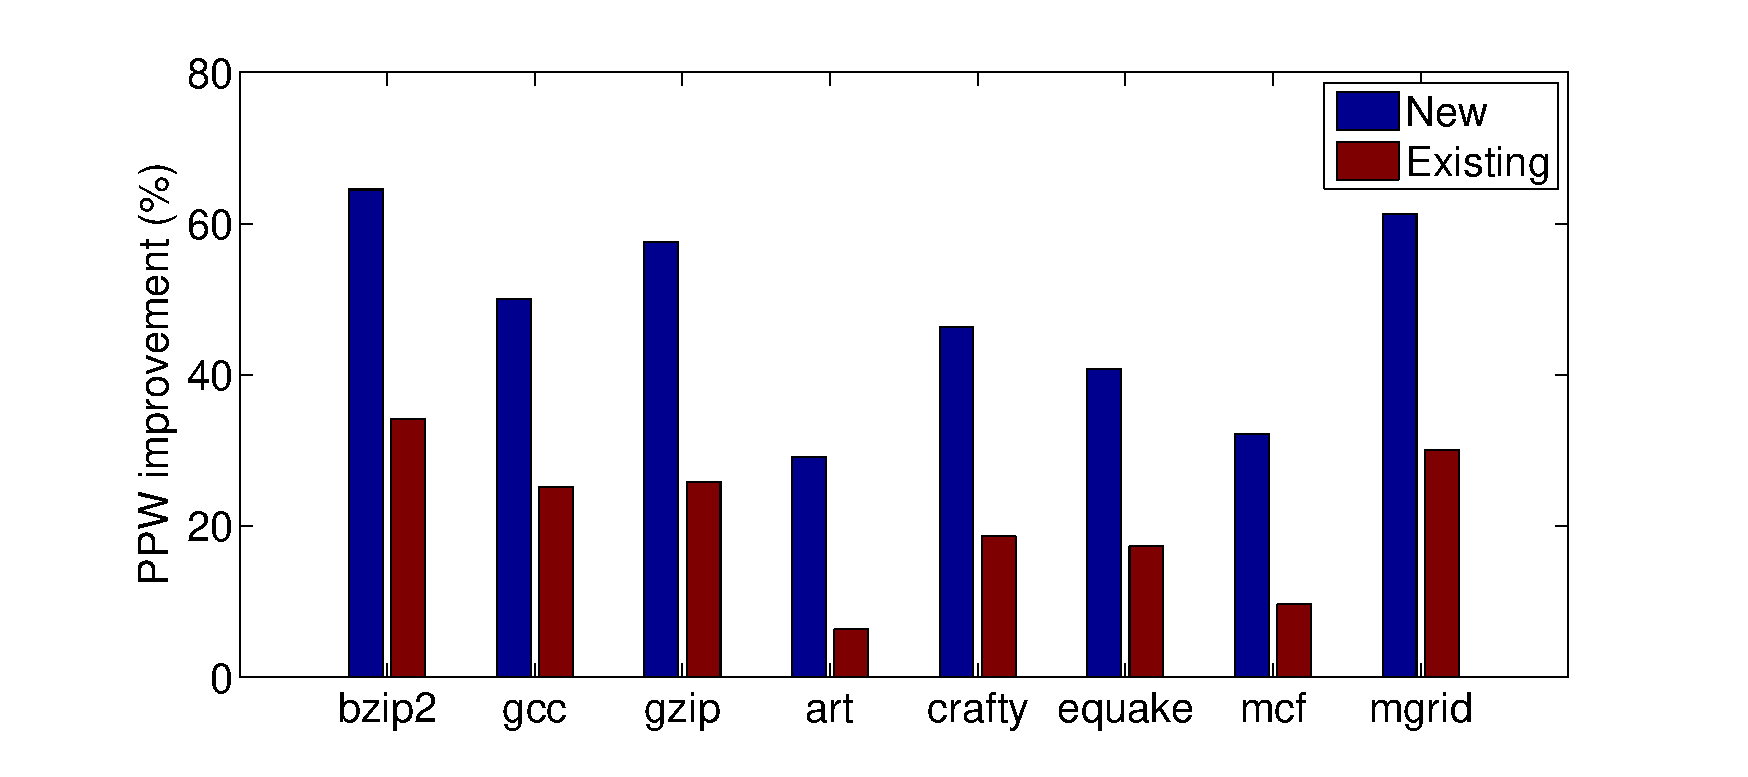
\includegraphics[width=1\linewidth]{fig/transient_ppw.eps}\label{fig:transient_ppw_spec}
\caption{PPW improvement comparison of new method and existing method.}
\end{figure}




